\section{Результаты}

\subsection{Задача 1}

Результат построения выпуклой оболочки случайных точек приведён на рисунке~\ref{fig:hull}. Красные точки являются вершинами оболочки, а синие точки лежат внутри или на границе полученного многоугольника.

\begin{figure}[H]
	\centering
	
\includegraphics[width=0.82\textwidth]{results/convex_hull_plot.png}
	\caption{Выпуклая оболочка 20 случайных точек}
	\label{fig:hull}
\end{figure}

Полученная фигура является выпуклым многоугольником. Действительно, \texttt{ConvexHull} строит наименьший выпуклый многоугольник, содержащий все исходные точки. Поэтому для любых двух точек внутри закрашенной области соединяющий их отрезок не выходит за границу оболочки. Это непосредственно соответствует определению выпуклого множества.

\subsection{Задача 2}

На рисунке~\ref{fig:sets} синим цветом показана часть круга $A$, не принадлежащая $B$, красным --- часть $B$, не принадлежащая $A$, фиолетовым --- пересечение $A\cap B$.

\begin{figure}[H]
	\centering
	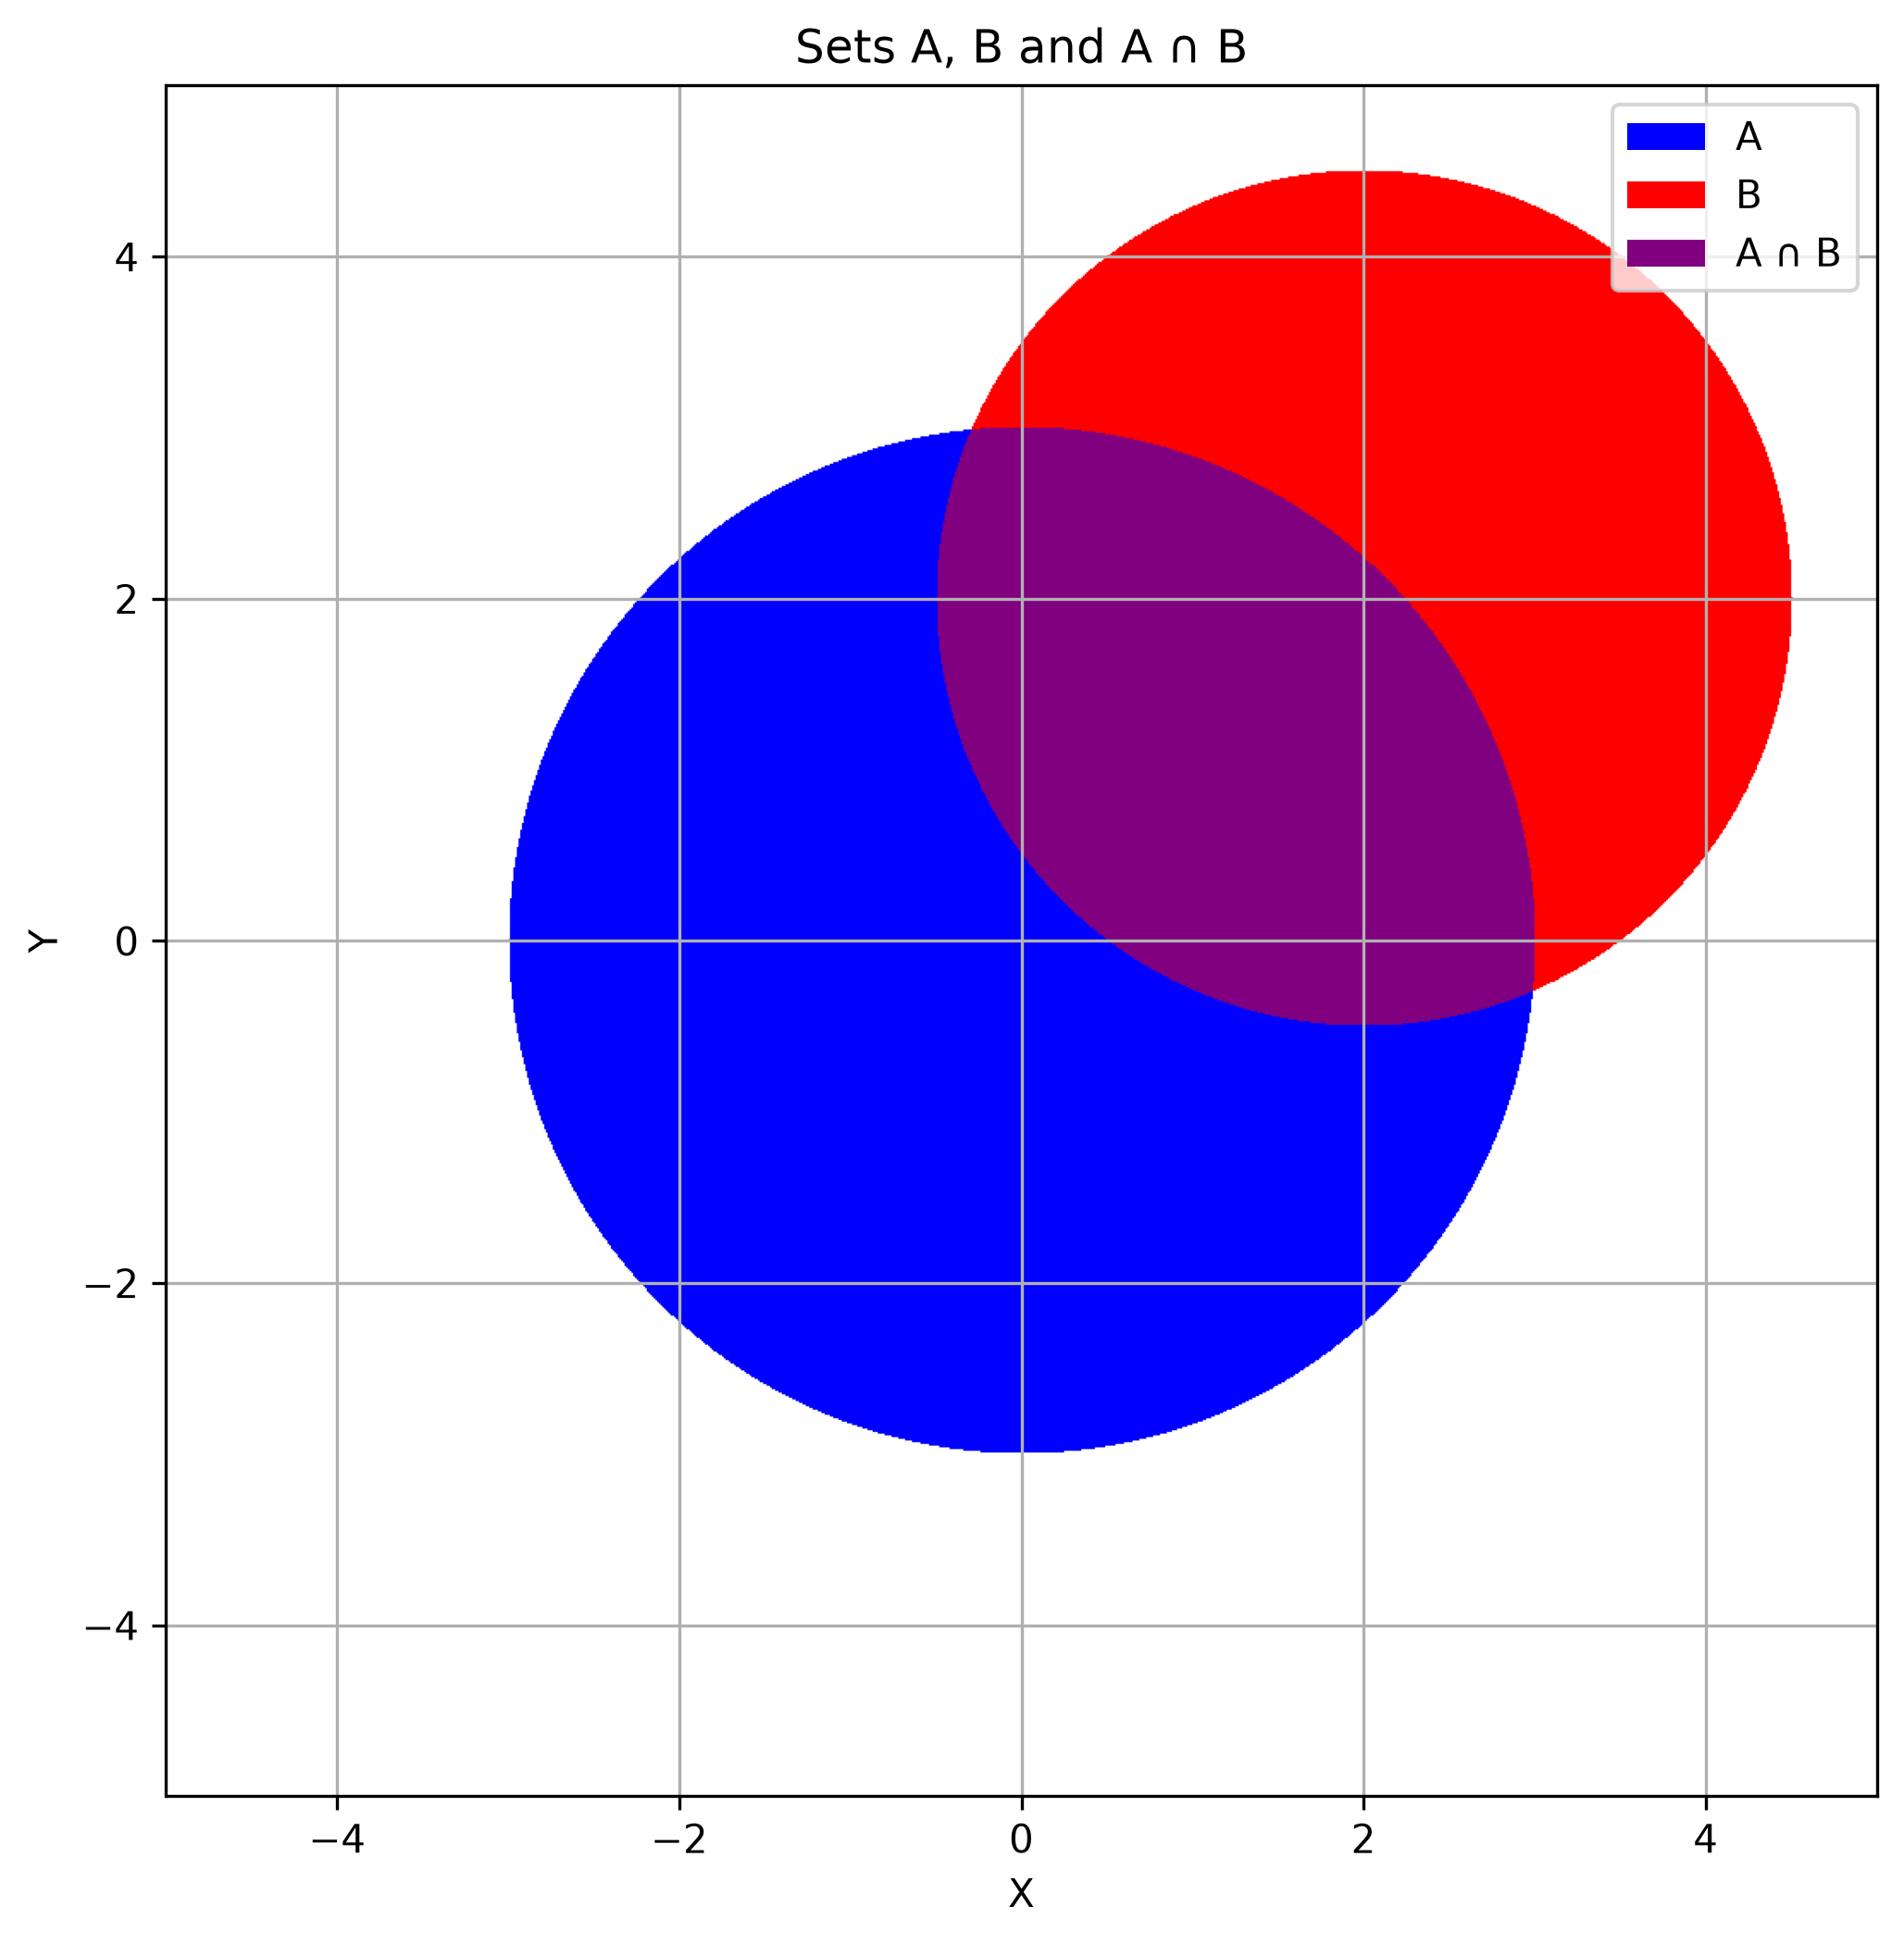
\includegraphics[width=0.78\textwidth]{results/sets_plot.png}
	\caption{Круги $A$, $B$ и их пересечение}
	\label{fig:sets}
\end{figure}

Оба круга выпуклы: для любых двух точек одного круга отрезок между ними также находится в этом круге. Их пересечение также выпукло по доказанному в теоретической части свойству. На графике фиолетовая область имеет форму линзовидного пересечения без выемок, что согласуется с теорией.

Следовательно, ответ на проверочный вопрос положительный: пересечение двух данных кругов является выпуклым множеством. Более того, пересечение любого числа выпуклых множеств всегда выпукло, хотя оно может быть пустым.

\subsection{Задача 3}

Результат печати программы:
\begin{verbatim}
True
False
False
\end{verbatim}

Первый результат соответствует выпуклому многоугольнику. В нём присутствует коллинеарная промежуточная точка и повтор первой вершины в конце списка, однако нулевые повороты игнорируются, а направление остальных поворотов сохраняется. Второй результат показывает, что многоугольник с выемкой невыпуклый: знак поворота меняется. Третий результат подтверждает невыпуклость звезды, у которой последовательные рёбра также дают повороты разных направлений.

\begin{figure}[H]
	\centering
	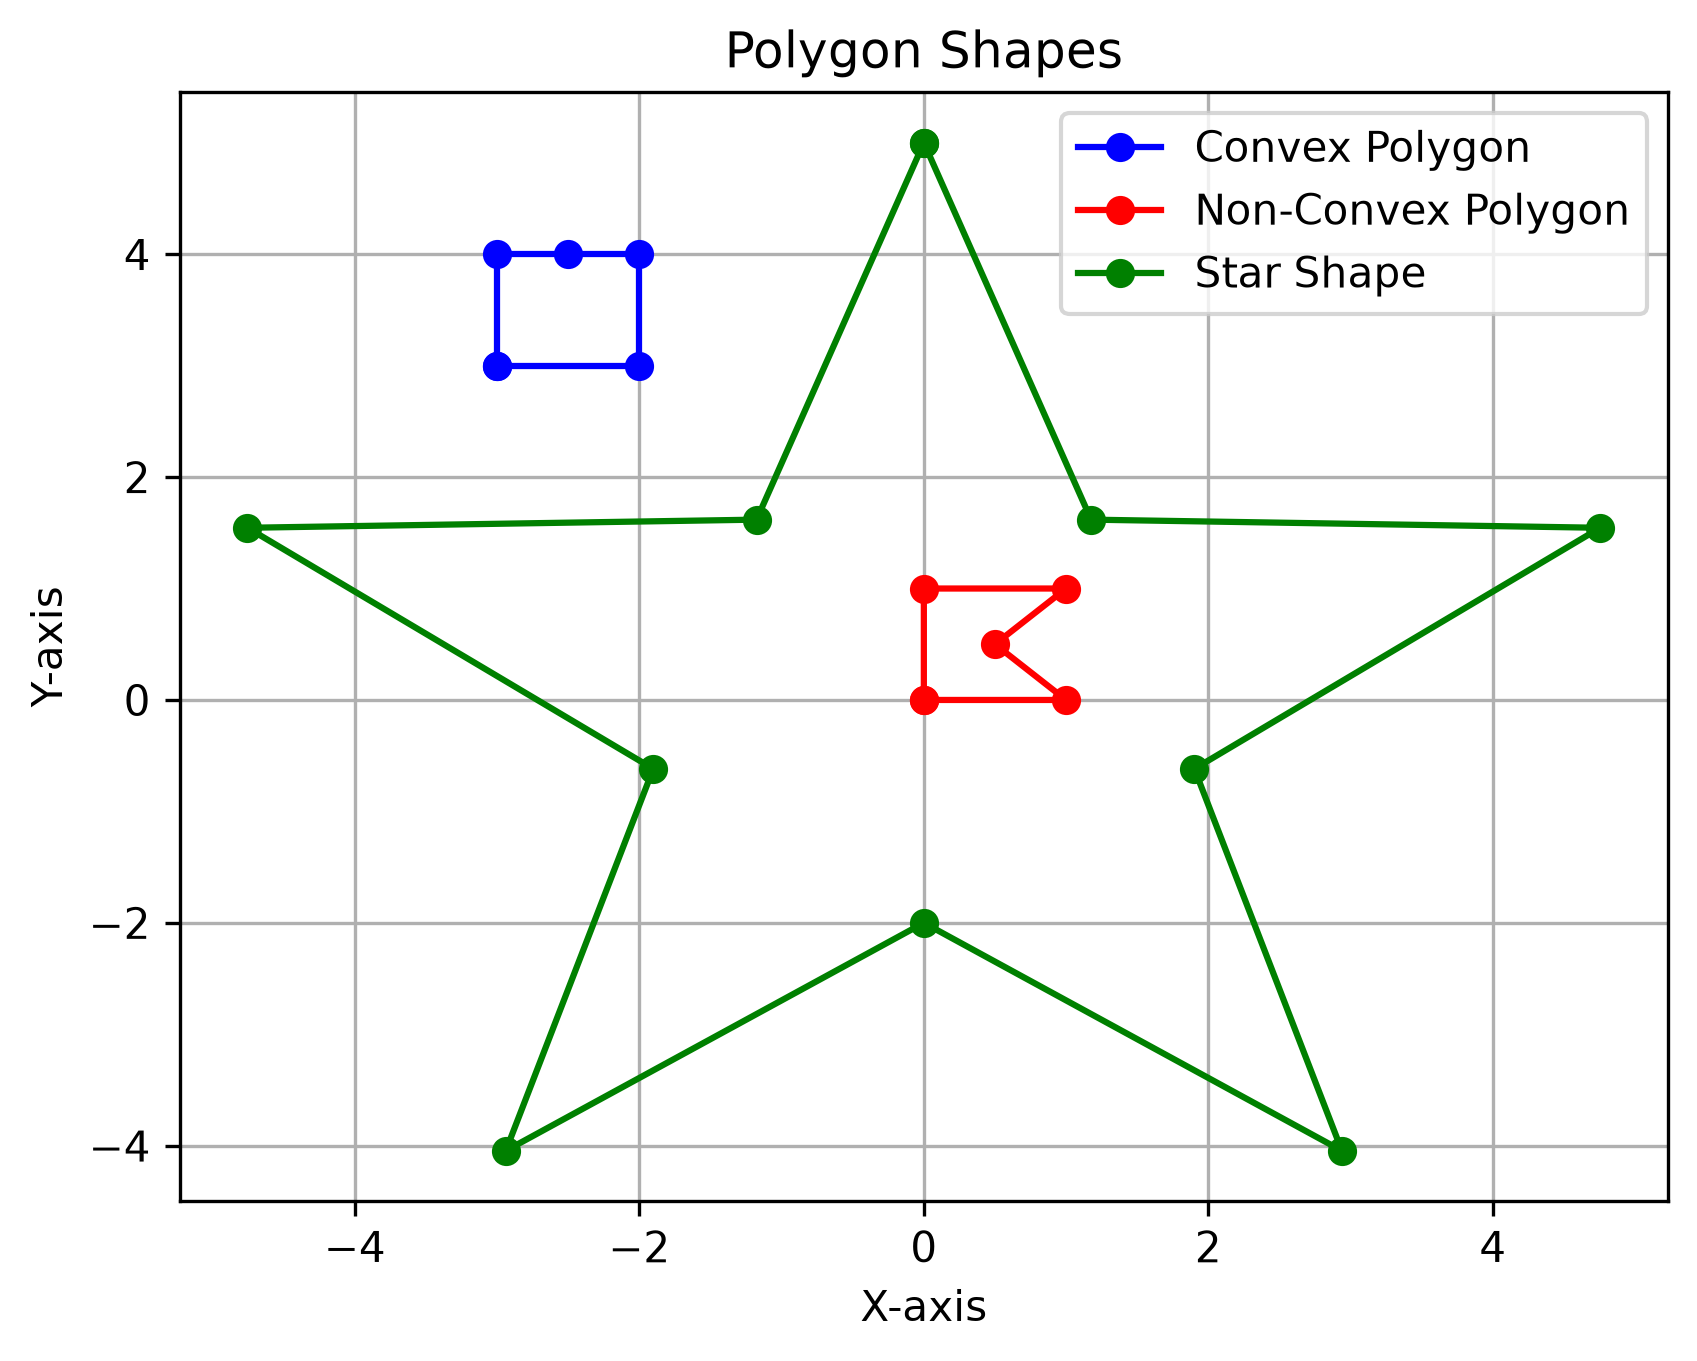
\includegraphics[width=0.82\textwidth]{results/convexity_tests.png}
	\caption{Фигуры, использованные для проверки критерия выпуклости}
	\label{fig:convexity}
\end{figure}

Таким образом, реализация критерия правильно различает выпуклый многоугольник, многоугольник с выемкой и звёздную фигуру на выбранных тестах.

\newpage
